%
% File naaclhlt2018.tex
%
%% Based on the style files for NAACL-HLT 2018, which were
%% Based on the style files for ACL-2015, with some improvements
%%  taken from the NAACL-2016 style
%% Based on the style files for ACL-2014, which were, in turn,
%% based on ACL-2013, ACL-2012, ACL-2011, ACL-2010, ACL-IJCNLP-2009,
%% EACL-2009, IJCNLP-2008...
%% Based on the style files for EACL 2006 by 
%%e.agirre@ehu.es or Sergi.Balari@uab.es
%% and that of ACL 08 by Joakim Nivre and Noah Smith

\documentclass[11pt,a4paper]{article}
\usepackage[hyperref]{naaclhlt2018}
%\usepackage[square,sort,comma,numbers]{natbib}
\usepackage{kpfonts}
%\usepackage{opensans}
%\usepackage{sourcesanspro}
%\usepackage[T1]{fontenc}
%\usepackage{PTSans}
%\usepackage{libertine}
%\usepackage{libertinust1math}
\renewcommand{\descriptionlabel}[1]{\hspace{\labelsep}\textsc{#1}}
%\renewcommand{\familydefault}{\sfdefault}
\usepackage{latexsym}
\usepackage{xcolor}
\hypersetup{
	colorlinks,
	citecolor=black,
	linkcolor=black,
	urlcolor=black}
\usepackage{booktabs}
\usepackage{amsmath}
\usepackage{amsfonts}
\usepackage{amssymb}
\usepackage{microtype}
\usepackage{todonotes}
\usepackage{graphicx}
\usepackage{fullpage}
\usepackage{xspace}
\usepackage{url} 
\usepackage{color}
\definecolor{harvardcrimson}{HTML}{A41034}
\definecolor{harvardgrey}{HTML}{B6B6B6}
\definecolor{harvarddarkgrey}{HTML}{808285}
\definecolor{harvardblue}{HTML}{0D667F}
%\aclfinalcopy % Uncomment this line for the final submission
%\def\aclpaperid{***} %  Enter the acl Paper ID here

%\setlength\titlebox{5cm}
% You can expand the titlebox if you need extra space
% to show all the authors. Please do not make the titlebox
% smaller than 5cm (the original size); we will check this
% in the camera-ready version and ask you to change it back.


\newcommand{\beer}{\textsc{Beer Prediction}\xspace}
\newcommand{\bplots}{\textit{bias-plots}\xspace}



%\newcommand\BibTeX{B{\sc ib}\TeX}

\title{\textsc{Using \beer on Personal Financial Data}  \\ {\small \color{harvarddarkgrey} Version 1.618}}

\author{Mark Kurzeja}

\date{}

\begin{document}
\maketitle
\begin{abstract}



Forecasting the future is hard. Forecasting ones financial future can be even harder. Using techniques from data mining, we introduce \textsc{Best Estimators of Economic Restraints} (\beer) to create an unbiased estimator of future cashflow requirements using a novel dataset of years worth of personal financial data from the author. With applications in personal finance, budgeting, retirement planning, and small scale prediction, these methods create nearly unbiased estimators of future outflows despite the data exhibiting sparsity, leptokurtosis, temporal correlations, and small sample-size observations. 

  
\end{abstract}

\section{Introduction} \label{sec:introduction}

\subsection{A Hypothetical Bet}

Imagine you and I are out for drinks. We go to the bar, and begin talking about predicting the future.  Annoyed with my optimism about prediction, you say to put my money where my mouth is, and you offer me the following bet:

\begin{quote}
	\textit{ \color{harvardcrimson}
	``Pull out a piece of paper. Write down the exact dollar amount that you think you're going to spend this month on anything you like. If you're right, within \$100, I'll give you \$1,000. Otherwise, you will owe me \$1,000''
	} 
\end{quote} 

Do you think I should take the bet? If the payoffs or tolerance were different should I take the bet? How would this change my spending in the short term? I'm at a bar, after all. Should I order a cheaper Busch Light instead of my favorite beer, a Blue Moon, to avoid the chance of going over? Would little changes like that make a difference? We will talk about the solution to this problem, in an optimal setting, in Section \ref{sec:problem} and exploring methods for prediction in Section \ref{sec:methodology} and Section \ref{sec:results}.

Wouldn't it be nice to predict spending in advance so that you don't have to wonder? Whether its to lessen the surprise of the unpredictable, or to decide what beer you're able to afford for the night, \beer aims to inform personal financial decisions in the short term for long term success. 

\subsection{Why Care?}

\newcommand{\budgetprob}{\textsc{Budgeting Problem}\xspace}
\newcommand{\preprob}{\textsc{Prediction Problem}\xspace}

Sometimes the consequences of not predicting your financial picture accurately can be devastating. Financial shortfalls quickly can lead to reliance on credit which often carries excessive interest rates and borrowing restrictions. If left unmanaged, this debt can quickly ``snowball'' and become significant in its own right. 

Financial surprises can shake even the most diligent budgeters, and so in order to begin assessing the impact of spending today on the financial future of someone tomorrow, a natural first step is towards the prediction of the needs of tomorrow. Prediction of the needs of tomorrow, if accurate, would allow one to adjust spending in real time to prevent overspending, and this would allow them to better plan out their financial future. 

This problem, of predicting the needs of tomorrow, is only a small part of a problem that I will call the This step of prediction is the first of a few steps that I aim to take to solve a problem that I call, more generally, the \budgetprob, and this will be explained in a lot more detail in Section \ref{sec:problem}. In Section \ref{sec:related_work} and Section \ref{sec:methodology}, I will go into how this problem has been approached by others and how I aimed to solve the prediction problem. In Section \ref{sec:results} I will discuss some of the methods that are a part of the \beer framework. 

\section{Problem Definition and Data} \label{sec:problem}

\subsection{The Budgeting Problem}
The prediction of future outflows is only a subset of a problem that I will call the \budgetprob. The \budgetprob is as follows:
\begin{quote}
	Imagine you have $D$ dollars to spend in a given time period of $T$ days. Conditional on having spent $C$ dollars so far (including future contractual payments), what is the probability that you will spend $x \in [0,\infty)$ in the next $T_d$ days assuming that you are prediction on day $T_b$.  
\end{quote}
This problem has several nuances, and it is best expressed in terms of an example. 
\begin{quote}
	Imagine David has \$2,000 dollars that he can spend in the month of January on all of his expenses. He sets aside \$800 for rent, a contractual payment, leaving \$1,200 left for variable spending. He has already spent \$200 in the first five days of the month, and so he has 26 more days until his budget resets. What is the probability that he spends only \$1 for the rest of the month? How about \$100? How about \$1,000 (he breaks even)? How about \$2,000 (he grossly overspends)?
\end{quote}

Using this framework, most of the problems in money risk management can be framed. In this case, the time frame, $T_d$ is 26 days and $T_b = 1/5/2018$. David has $D = \$2,000$ to spend at the beginning of the month, has spent $C = \$1,000$ within the first five days, and so he has $D - C = \$1,000$ left to spend for the remaining $T_d$ days. 

More mathematically, we are trying to approximate the function:
\begin{align*}
P(X | T, D, C)
\end{align*} 

\newcommand{\custompartial}{\ensuremath{\hspace{-3mm}\partial x \hspace{2mm}}}
The probability of overspending, for example, is now the probability of spending greater than $D - C$ dollars in the next $T_d$ days which can be expressed as:
\begin{align*}
\int\limits_{D-C}^{\infty} \hspace{1mm} \custompartial P(X | T_b, T_d, D, C) 
\end{align*}
and the probability of spending within \$100 of your goal, as we posited as a hypothetical bet in Section \ref{sec:introduction}, can now be expressed as: 
\begin{align*}
\int\limits_{D - 100}^{D + 100} \custompartial P(X | T_b, T_d, D, C) 
\end{align*}
Using the math of the \budgetprob, one could figure out what the optimal decision is to the hypothetical bet in Section \ref{sec:introduction} is when combined with a loss function. 

Despite the great properties of this function, it is \textit{very} hard to estimate in practice. This is the golden standard of all prediction in personal finance. To make this problem tractable, we will instead deal with a subset of the \budgetprob, called the \preprob to gain insight into this. 

The \preprob is a subset of the \budgetprob as defined above. The \preprob assumes the following:\

\begin{enumerate}
\item $T_b \perp X$: each time period, with respect to prediction, is independent of $X$, equivalent to any other time period beginning, and not important to the prediction of $X$. This is a temporal independence assumption that ignored changing prediction patters to ensure that the sparsity of the data is somewhat combated. 
\item $T_d = 30$: the \preprob focuses on a 30 day lookahead prediction
\item $C = 0$: there has been no contractual spending for the month assumed and no spending we need to account for in the beginning of the month that will be added to $X$
\item $D \perp X$: $D$ will be assumed to be independent of $X$. This, in reality, is an assumption that may not hold since your spending habits would be expected to change given the amount of money that you have to spend. 
\item The expectation of $X$ contains all of the information about $X$. Some methods will allow us to model the variance of the expectation of $X$, but they will not allow us to estimate the variance of $X$ directly. In the instances where the variance of the expectation of $X$ is difficult or impossible to find conditional on a model, we will have to assume the variance of the expectation of $X$ is zero
\end{enumerate}

In this way, the \preprob is, at its very heart, a ``best prediction'' of the variable spending of someone under loose independence assumptions of monetary constants. This is a key insight and is necessary to understanding why the dataset was chosen in the way that it was. 


Thus, we are trying to solve the following with the \preprob
\begin{align*}
\mathbb{E}_X\left[ P(X | T = 30, D, C = 0) \right]
\end{align*}
which by the independence of $D$ and $X$ is equivalent to
\begin{align*}
\mathbb{E}_X\left[ P(X | T = 30, C = 0) \right]
\end{align*}


\subsection{Issues with the Data}
In this way, we are solving each of the issues in the data with the following:
\begin{description}
	\item[Sparsity] There are many days in a row that I will not spend any money. In this way, only about 25-30\% of the time series is non-zero which means that the length of the time series is not a good indication of the amount of data
	\item[Leptokurtosis] If we think about the kurtosis of a normal distribution, it is three. A t-distribution with 2-4 degrees of freedom has a kurtosis of six. My data has a kurtosis of twenty-two which means that it is characterized by a large amount of spurious activity that is very difficult to characterize, and outliers tend to dominate the data
	\item[Temporal Correlations] When I spend money, some parts of the year I tend to spend quite a lot of money and some parts of the year I will not spend anything. This tendency of the spending to "cluster" tends to indicate that spending habits exhibit short term and sometimes long term correlations. 
	\item[Small Sample Size] At the end of the data, this data is expensive in time to gather. If we need to get 1,000 data points to accuracy predict spending, I will need to wait almost three years to make predictions for most individuals. The challenge is to use as little data as possible to predict measurements, and as a result, the largest challenge, besides the challenges above is how to work with small sample sizes in generalizing predictions for the highest degree of accuracy. 
\end{description}

\subsection{Evaluation Metrics}
For this analysis, the evaluation method that I will use are \bplots. These plots the length of the training data that is used in a prediction against the average lookahead error that each of these have. 

First, we get the error data using the following method:
\begin{enumerate}
	\item Let $ l \in \left[ 5, 800 \right]   $ be the length of the training set. 
	\item Let $ t_b $ be the beginning of the training set. So the data that we will train on will be from $ \left[ t_b, t_b + l \right]  $ inclusive
	\item Let $y $ be the sum of the expenditures from $ \left[ t_b + l + 1, t_b + l + 30 \right]  $. This is the 30 day look ahead value
	\item Train a model on the training data and generate a prediction $ \hat{y} $ for $ y $. 
\end{enumerate}
Then we will take this data and do the following to generate the plot
\begin{enumerate}
	\item Group the data by each $ l $ and compute the arithmetic mean error of all of the $ \hat{y} $
	\item For each $ l $, plot the mean error
\end{enumerate}
This plot can be useful for interpreting several features of each algorithm:
\begin{description}
	\item[Unbiasedness] If an algorithm is unbiased, especially for lots of sizes of training data, then we will see that the average of the errors will be approximately zero across the entire plot. That is, if all of the points are on the x-axis, in the range of $ l $, then the algorithm is unbiased. If there is any deviation from this line, then it means for that number of training points, the algorithm was systemically over or under predicting the real result.
	\item[Best Training Size] For this particular dataset, what is the best size of training data to use? Can we get away with only training on 50 data points or do we need 200 data points in order to sufficiently train the model
	\item[Autocorrelation] Are the errors in the model autocorrelated? Are there parts of the training space that are very difficult to predict, or is this something that is random and essentially Gaussian style noise? How the points are plotted, and how they vary around the mean, give us an indication of this.  
\end{description}




\subsection{The Data Set}
I have every single dollar tallied that I have spent in the past few years in my budgeting program. The data for a transaction includes the following:
\begin{description}
	\item[Date] The Date the transaction took place
	\item[Account] From which of my personal accounts did the money come from? Checking, Savings, Etc?
	\item[Master Category] A high-level category assigned by myself. This includes things like is this a Housing Expense? Is this a Leisure Expense? Is this a Financial Expense? etc.
	\item[Sub Category] This is a more granular category that is meant to break up the master categories. If something is a housing expense, is it for rent, or household items, or for a security deposit?
	\item[Payee] Who was the transaction to?
	\item[Outflow] If the item was an outflow, what was the amount?
	\item[Inflow] If the item was an inflow, what was the amount?
	\item[Memo] User-generated description of the expense
\end{description}

Further to each of the data points above, I have the total amount spent in each category during the last five years and I can see how I planned for expenses in the future using the data from my budgeting values. 

The dataset that I am working with is 2625 transactions spread across several years worth of data. I am currently working on integrating older data as well which will get the dataset to be around 4000 transactions in total, but as of right now, the dataset will remain at 2625 transactions. Since my problem inherently is a time-series prediction problem using sparse data, it is a continuous regression problem and with transaction data as granular as daily, I have a lot of features that I have been working to engineer for the dataset including running averages, lag period prediction, and other methods that may improve the prediction on the coming months.

Some of the most frequent features of the data include severe outliers and large periods of days where there are no transactions to note. When I lived in New York, there were entire month periods where I didn't eat much at all at a restaurant, and as a result, those months appear as dead-months in the dataset. Similarly, if I was out for my girlfriends birthday at the time, then I would see that this shows up as a clear outliers in the dataset. It is these sporadic measurements that make this a difficult prediction problem even for mean estimation and this is something that I am working on trying to figure out. 

The data is as clean as my recording has been over the last three years. Since this register is tied to the cent to my bank accounts every week, I know that the data is good and it should be very clean, but the only information that I have on each transaction, other than the parties involved and the month, are the comments that I leave and there are many of them without a comment in the dataset. An example of the data is contained in Table \ref{exampledata}.
\begin{table*}
	\resizebox{\textwidth}{!}{  
		\begin{tabular}{cccccccc}
			Account         &   Date    &     Payee     & Master Category &        Sub Category        &      Memo       & Outflow & Inflow \\ \midrule
			Capital One Quicksilver & 8/13/2016 & Diner Airport &  Everday Wants  & Partying, Drinks, and Food &  Food airport   & \$24.04 & \$0.00 \\
			Capital One Quicksilver & 8/13/2016 &   Quik Fill   &  Everday Wants  & Partying, Drinks, and Food &    Trip tea     & \$1.38  & \$0.00 \\
			Cash In Wallet      & 8/20/2016 & Jakes Saloon  &  Everday Wants  & Partying, Drinks, and Food & Justin and Pete & \$27.00 & \$0.00 \\ \bottomrule
		\end{tabular}
	}
	\caption{Three Data points from the data set}
	\label{exampledata}
\end{table*}

\begin{figure}
	\centering
	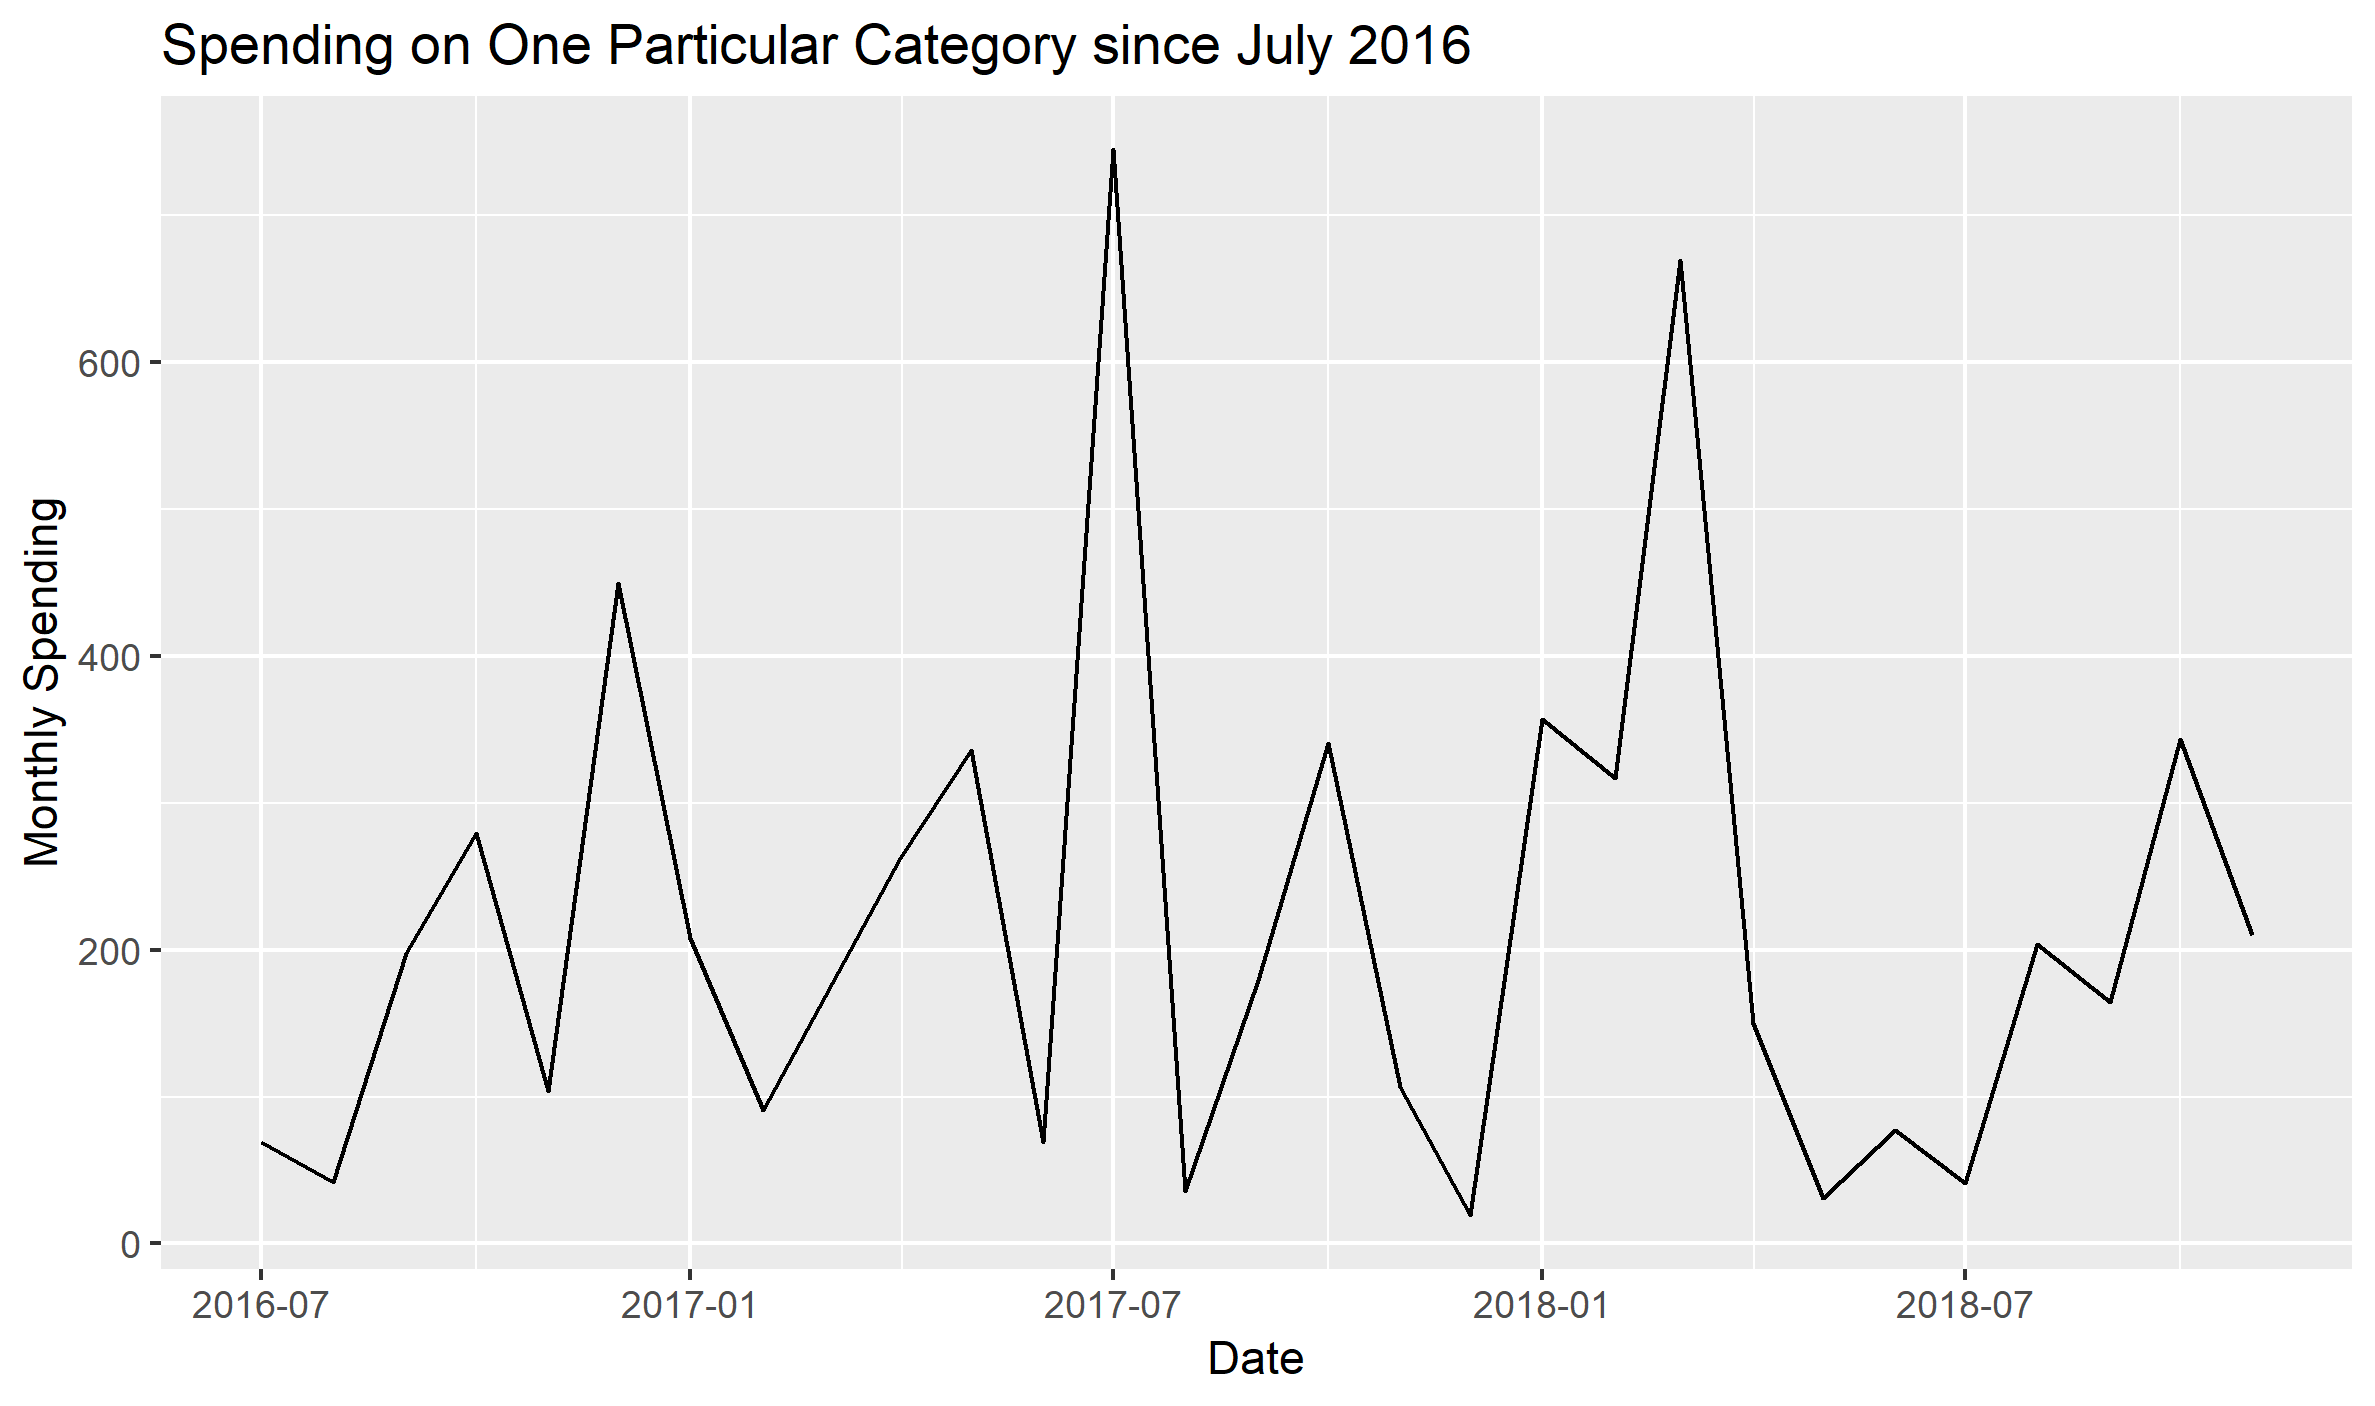
\includegraphics[width=0.7\linewidth]{../figures/Spending_Example}
	\caption{Monthly aggregation of spending for a particular category}
	\label{fig:spendingexample}
\end{figure}
	
	


\section{Related Work} \label{sec:related_work}

There has been a lot of work on personal forecasting but most of it, to maintain simplicity, has been based off of using simple averages and running averages to predict the spending in the coming months. 


The prediction problem for time series is well studied however, and from that perspective there are a variety of methods that have been brought to the table. Anything from ARIMA modeling to Facebook's Prophet have been found to be useful. Gaussian Processes are something that may be useful to get variance estimates for each of the predictions, and other models that allow for smoothing of noisy data may be useful as well. ASAP, which we saw in class, is something that may be able to take out a large variety of the variation that financial data often brings about as well. 

In \cite{SVMFinance}, the authors used SVM, training on several properties of the time series up until this point, to predict how the stock will develop in the coming months. For this projects, I could use similar features such as volatility in the previous periods as well as skew and other technical oscillators borrowed from technical finance such as the Relative Strength Index and the Commodity Channel Index to use as training features and then run supervised machine learning algorithm on the data. In this way, I could hope to get away from the nature of the time-series modeling I have been doing in order to begin creeping into the more classical approaches to prediction treating the new monthly average as a predictive of the previous months. 

In \cite{LongTail}, the authors used extreme-value modeling to come up with predictions of tail-risk in their financial modeling. Looking at my project from this lens, this is the measure that I am trying my hardest to estimate. Seeing as most people don't really care about the expected value of their spending, but rather would like to know the maximum for risk modeling, this paper actually may have changed my problem statement for some of the modeling a little bit. I would like to explore how to use these models to better estimate tail risk, and I want to build a model that is able to account for the tail risk of my spending. 


\section{Methodology} \label{sec:methodology}

\subsection{Data Processing}
There were several data preprocessing methods that were chosen to facilitate prediction and allow for new 

\newcommand{\yinyang}{\textit{Yin-Yang}\xspace}

\begin{description}
	\item[Raw Data] Many of the algorithms were tested using the raw data as a sequence. This was done to see if many of the algorithms could actually handle the data without further processing
	\item[Autoregressive Data] Autoregressive matrices were built off of training sequences for prediction models. This method was used to discern if there was any improvement that advanced prediction methods could bring to the time series prediction task behind the \preprob
	\item[\yinyang Data] I used a custom processing method that I will call the \yinyang Method for prediction Because much of the data consists of a spending measure and then a series of zeros and then another transaction and another series of zeros, \yinyang prediction aims to take the training data and build from it a series of the following form: $(Amount_t, Zeros_t) \rightarrow (Amount_{t + Zeros_t}, Zeros_{t + Zeros_t})$. In this way, the sequence of spending of $30, 0, 0 , 0 , 5, 10, 0, 0 , 2$ would be transformed into $(30, 3) \rightarrow (5,0) \rightarrow (10,2)$. Then methods were used created to take in a tuple of size two, like these and predict the next tuple in the sequence These \yinyang methods aimed to take advantage of the data generating process of spending followed by sometime until the next purchase
	
\end{description}

\subsection{Description of Models}
There were a variety of methods that were used on the data including the following models:
\begin{description}
	\item[ARIMA] ARIMA implementation used in base R with default parameters
	\item[GLM] Generalized Linear Model ran using GLM in R with default settings
	\item[SVM] E1071 SVM implementation in R using default settings with linear, radial, and polynomial kernels
	\item[Random Forests] R implementation of Random Forests using default parameters
	\item[Decision Tree] Decision trees from the Rpart package in R using default parameters
	\item[Prophet] Facebook's Prophet Algorithm \cite{Fbook} as implemented in R
%	\item[label] description
\end{description}

\subsection{Bringing Data and Models Together}
In each case, the models will be evaluated in the holdout error for the time series aimed to be estimates of a statistical measure known as \textsc{LOO} - this is the leave-one-out cross validated error and it is one of the best measures of prediction error out-of-sample.

For the raw data, the algorithm was as follows:
\begin{enumerate}
	\item Pick an algorithm of choice
	\item Pick a starting point $ t_b $ and a size $ l $ of the training data
	\item Let $ T $, the training data, be the spending from $ t_b $ to $ t_b + l $
	\item Train, using the raw data with zeros, the algorithm on $ T $
	\item Let $ V $ be the sum of the data from $ t_b + l + 1 $ to $ t_b + l + 30 $. This is the actual amount of spending
	\item Run the predictions forward 30 days recursively using the new estimates to inform the next prediction. Let $ \hat{V} $ be the sum of thirty days worth of predictions
	\item Predict $ \hat{V} $ using the trained algorithm and let the error of the observation be $ \hat{V} - V $
	\item Repeat this process for a large number of choices for $ t_b $ and $ l $ and for every algorithm under consideration
\end{enumerate}

For the autoregressive models, the algorithm was as follows:
\begin{enumerate}
	\item Pick an algorithm of choice
	\item Pick a starting point $ t_b $ and a size $ l $ of the training data
	\item Let $ T $, the training data, be the spending from $ t_b $ to $ t_b + l $
	\item Transform $ T $ into an autoregressive matrix with 20 lags as the covariates That is, the first line is: $$ T_{t_b + 21} = f(T_{t_b + 20}, T_{t_b + 19}, \ldots , T_{t_b + 1}) $$ The second line begins with $ T_{t_b + 22} $ and is predicted with $ T_{t_b + 21} \rightarrow T_{t_b + 2} $ and so on and so forth
	\item Train, using the autoregressive data, the algorithm on $ T $
	\item Let $ V $ be the sum of the data from $ t_b + l + 1 $ to $ t_b + l + 30 $. This is the actual amount of spending
	\item Run the predictions forward 30 days recursively using the new estimates to inform the next prediction. Let $ \hat{V} $ be the sum of thirty days worth of predictions
	\item Predict $ \hat{V} $ using the trained algorithm and let the error of the observation be $ \hat{V} - V $
	\item Repeat this process for a large number of choices for $ t_b $ and $ l $ and for every algorithm under consideration
\end{enumerate}

For the autoregressive models, the algorithm was as follows:
\begin{enumerate}
	\item Pick an algorithm of choice
	\item Pick a starting point $ t_b $ and a size $ l $ of the training data
	\item Let $ T $, the training data, be the spending from $ t_b $ to $ t_b + l $
	\item Transform $ T $ into a \yinyang sequence using the process described in the \yinyang data procedure
	\item Train, using the \yinyang procedure and a Markov assumption on transitions, the algorithm on $ T $
	\item Let $ V $ be the sum of the data from $ t_b + l + 1 $ to $ t_b + l + 30 $. This is the actual amount of spending
	\item Compute predictions on the \yinyang sequence forward until the number of days covered (tallied though the number of days with zeros) is greater than or equal to 30.
	\item Predict $ \hat{V} $ using the trained algorithm and let the error of the observation be $ \hat{V} - V $
	\item Repeat this process for a large number of choices for $ t_b $ and $ l $ and for every algorithm under consideration
\end{enumerate}

Using all three of these data processing methods, I generated the final \bplots for the report which then can be used to access the error. 

\section{Evaluation and Results} \label{sec:results}

\newcommand{\lookback}{\textit{Look-back Averaging}\xspace}

\subsection{Naive Models}

Before a presentation of errors for more advance models is presented, a more simplistic baseline first has to be established using both ARIMA models and \lookback. ARIMA models are common in time series analysis, and so they are a natural place to start. Look-back averaging uses the average of the last $k$ points linearly scaled as the best prediction of the look-forward average. The \bplots of both methods are presented in Figure \ref{fig:08nullerrors}.

The top two plots show the errors of the methods without averaging, and the bottom shows them averaged for each of the training data sizes. We can see that for low amounts of training data, both ARIMA and \lookback both have almost unbiased error. This somewhat makes sense since spending tends to have a mean structure that doesn't vary too quickly with time. However, if we look at the top plots, we can see that the error for small predictions, while unbiased on average, are sometimes as large as 600. Since the scale of the spending is often around \$300-\$500 a month, this level of error is unacceptable and other methods will aim to reduce the variance of the errors as well as keeping the unbiased property of these algorithms at small sample sizes.

An interesting trend with the ARIMA and \lookback data is the auto-correlation that training sizes from 400-800 exhibit. Since they are both using expectations, it appears to be the case that having too much information to train on (e.g. taking a long term average instead of a short term average for prediction) tends to actually bias the estimates up which causes the algorithms to be unbiased overall as they gain more training data. This was surprising for ARIMA as I expected it to pick up on this trend, but it did not. The moral of the story with naive methods is that less may be more in training data, but the cost of this is excessive variance. 

\begin{figure}
	\centering
	\includegraphics[width=1\linewidth]{../figures/08_null_errors}
	\caption{Null Model Errors}
	\label{fig:08nullerrors}
\end{figure}
	
\subsection{Autoregressive Methods}

When we run use the autoregressive modeling setup, the modeling problem becomes a prediction problem where the lags are now the covariates. I trained six models and then recorded their error for each training size. The raw errors can be seen in Figure \ref{fig:arerrorswzeros} and the means of the errors can be seen in Figure \ref{fig:arerrorswzerosmeans}.

Each of the models were trained using lags of sized 20 for the data, and their results are as follows:
\begin{description}
	\item[Decision Trees] Decision trees were fit on the autoregressive data. Out of the various methods, the decision trees had the largest true error of over \$1,500, and this variance makes them unpractical for use. The algorithm was downwards biased from 0-600 training size and then upward bias after this range. 
	\item[GLMs] Generalized Linear Models were relatively unbiased from training sizes of 0-400, but were upward bias past that training size. Out of the models considered, they were the only model that was largely unbiased on average for a majority of the training sizes, which indicates that they are able to outperform the other models considered in the autoregressive context for this data
	\item[Random Forests] Random Forest were trained on the autoregressive data. While the variance is not as large as the decision trees, they systemically were upwards bias, and for no size of training data were they ever unbiased estimators of next months spending
	\item[Support Vector Machines] Using the Linear, Polynomial, and Radial Kernels for SVM on the autoregressive data yielded largely similar results. The SVM was downwards biased for all input sizes, and this performed the worst out of all of the models considered for autoregressive prediction. 
\end{description}


\begin{figure}
	\centering
	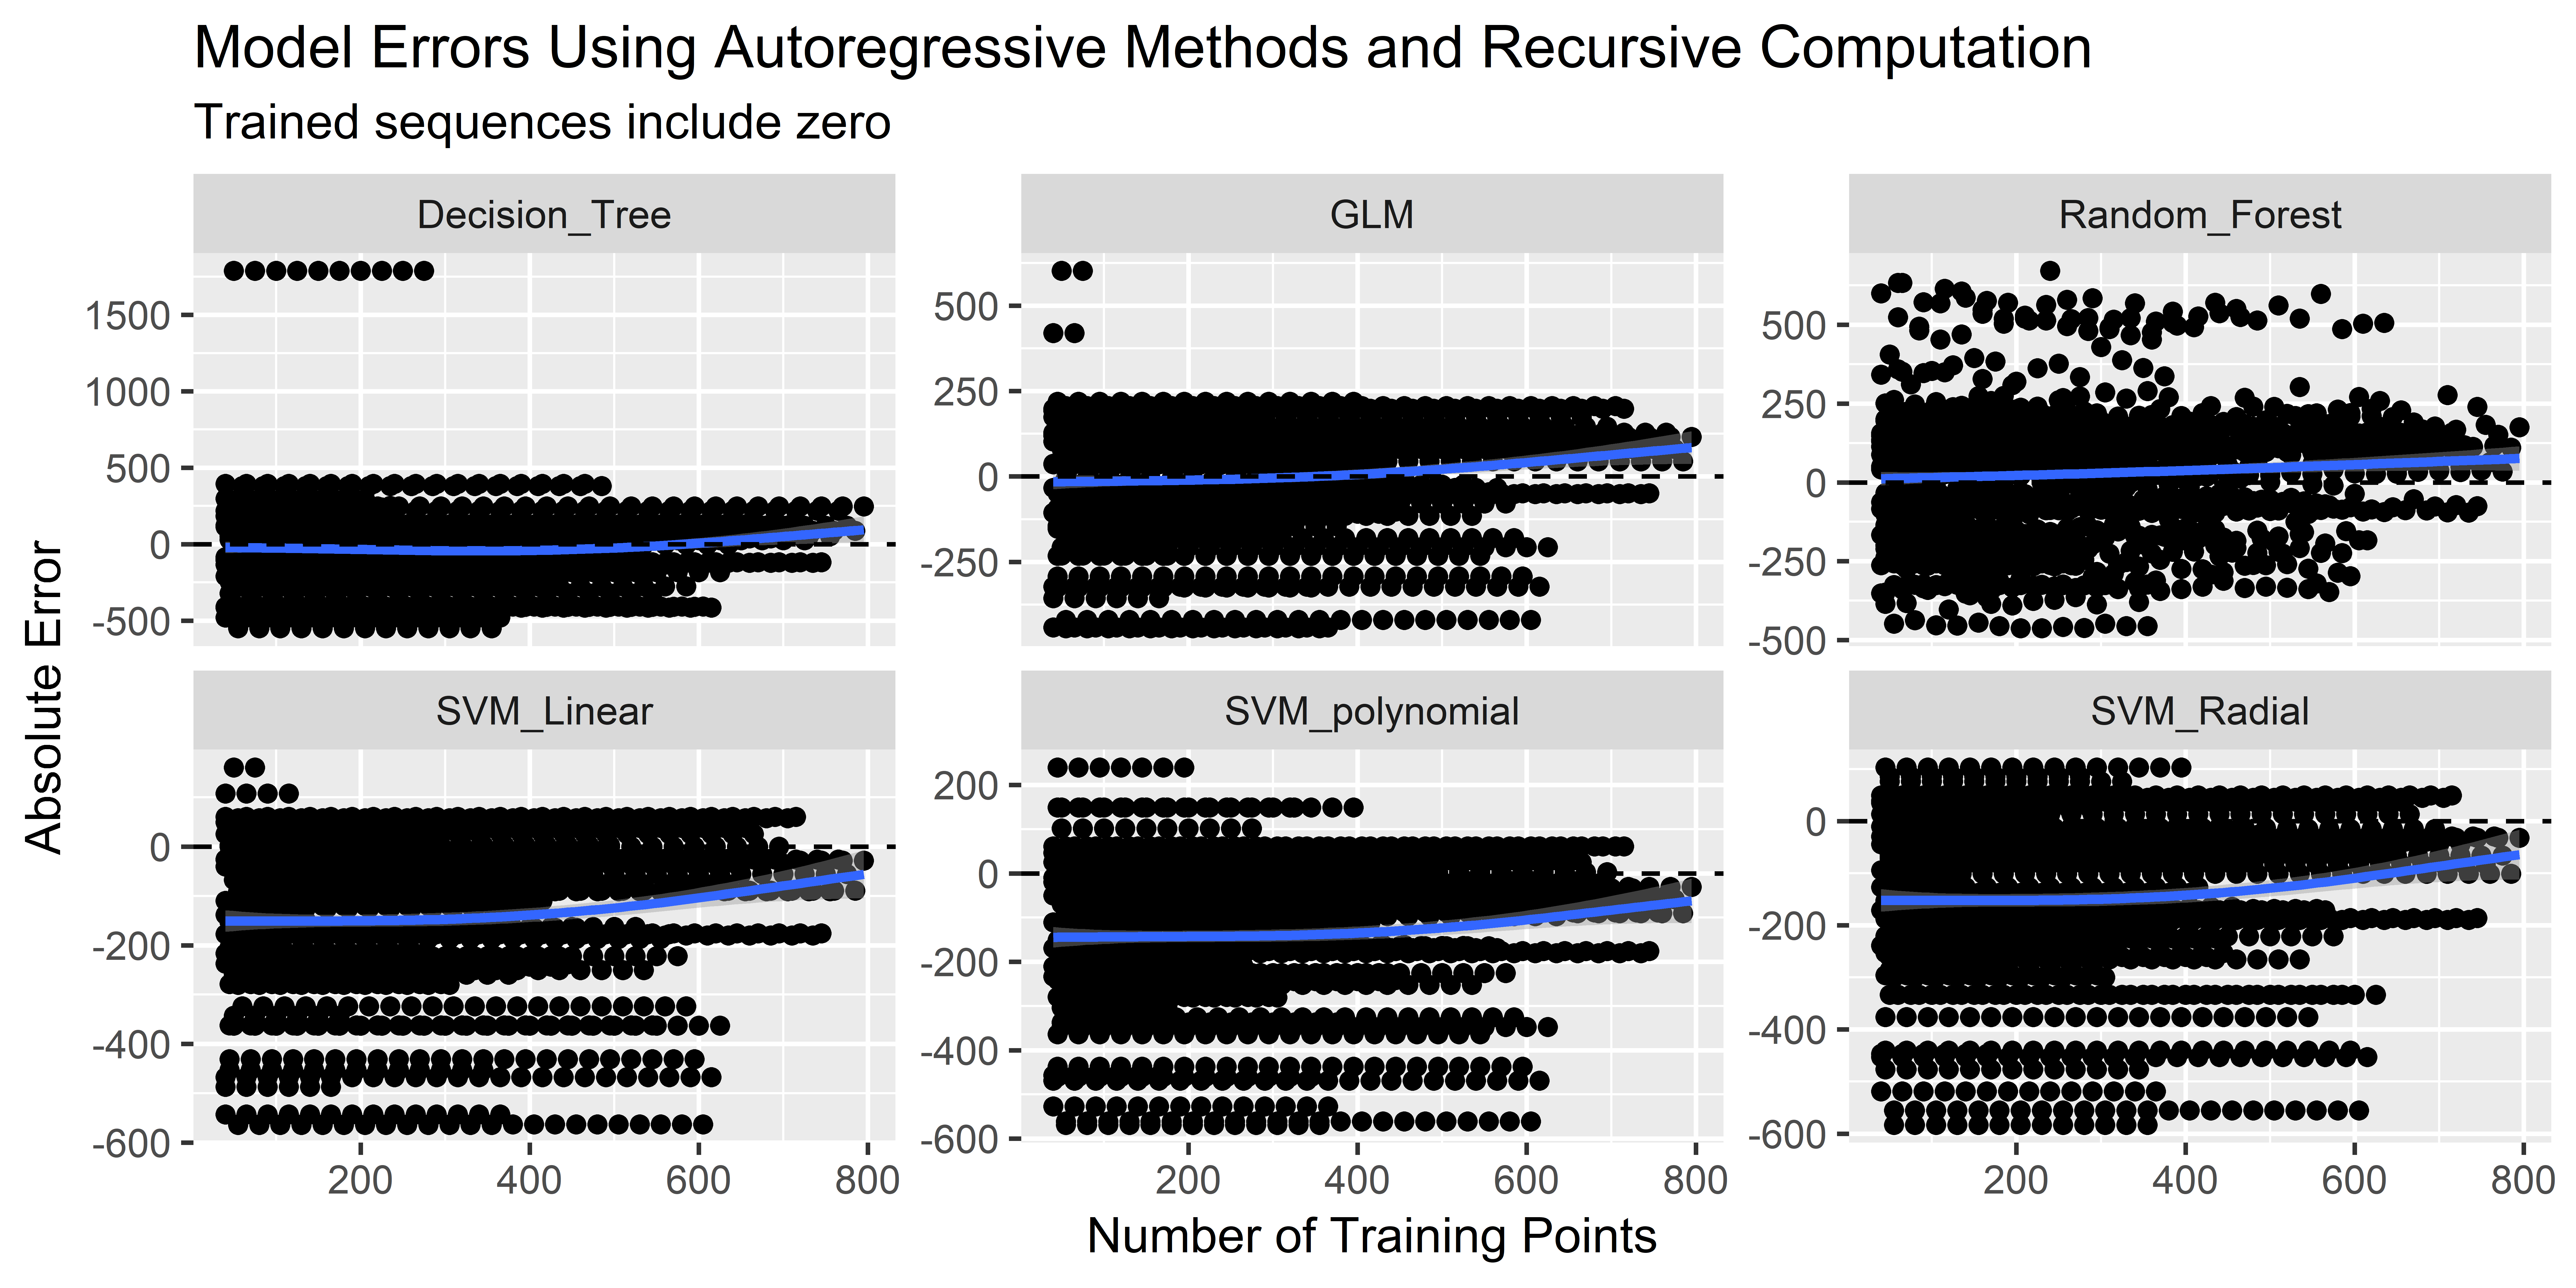
\includegraphics[width=1\linewidth]{../figures/ar_errors_w_zeros}
	\caption{Autoregressive errors for each training size}
	\label{fig:arerrorswzeros}
\end{figure}

\begin{figure}
	\centering
	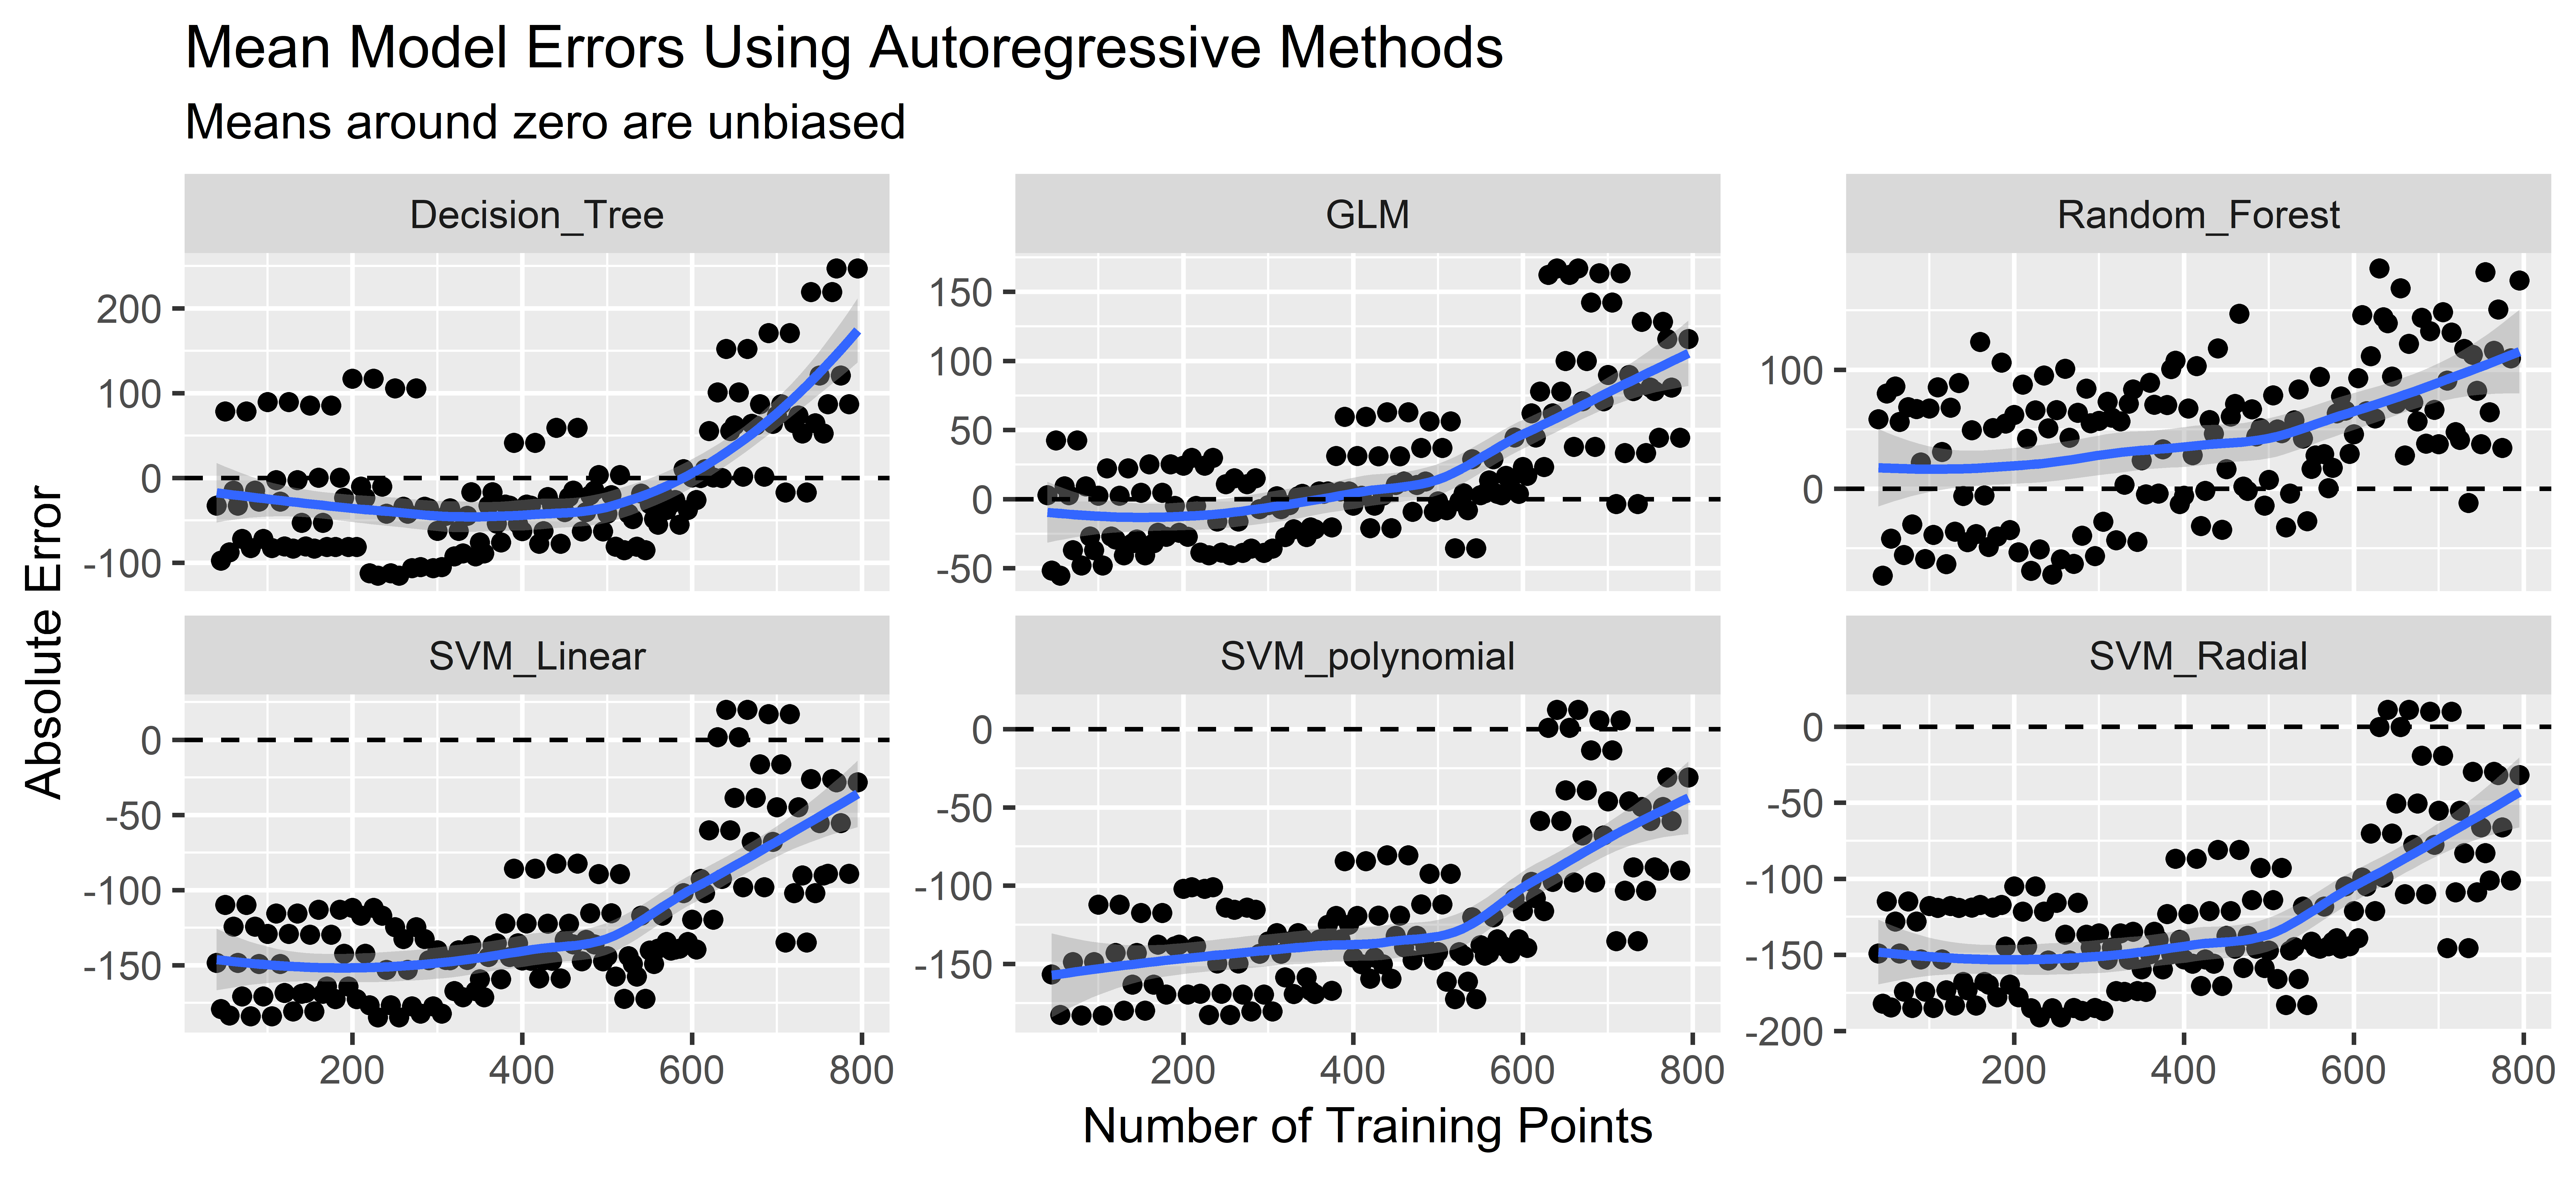
\includegraphics[width=1\linewidth]{../figures/ar_errors_w_zeros_means}
	\caption{Autoregressive mean errors for each training sequence size}
	\label{fig:arerrorswzerosmeans}
\end{figure}




\subsection{Yin-Yang Regression}
\yinyang data prediction, as described in Section \ref{sec:methodology}, amounts to a Multivariate regression problem that aims to predict, given a spending amount and the time between this and their last expenditure, how long it will be until they spend money and what that amount will be. 

In this prediction, we are aiming to find a function $f$ such that 
\begin{align*}
f(x_1, x_2) \rightarrow (y_1, y_2)
\end{align*}
However, most algorithms only output one value for their predictions. I combated this by one of the following two methods:
\begin{enumerate}
	\item I estimated the spending amount and the count amount independently using past data and then used this for the next prediction value. This method works well, but it does not take into account the fact that often there is a correlation between how much is spent and how long it is in between visits. For example, imagine that you spend a lot on groceries. This large amount spent will likely last longer. This means that there is a corresponding positive correlation between amount spent and the number of days that will occur before the next time that groceries are purchased
	\item To decouple the correlation between spending and the number of zeros following it, I ran PCA in the second method to attempt to decouple the correlation between the variables, predicted using the scores in the PCA space, and then re-transformed them back onto the original coordinates for predictions
\end{enumerate}

If we look at Figure \ref{fig:07yinyangmultiple}, we can see that the GLM method was upwards biased for every amount of training data in the set. This also applies to the PCA transformed \yinyang data. This should make sense since PCA is essentially computing a linear transform of the data, and the GLM is taking a linear function of the inputs to predict the outputs so we should expect similar results. 

\begin{figure}
	\centering
	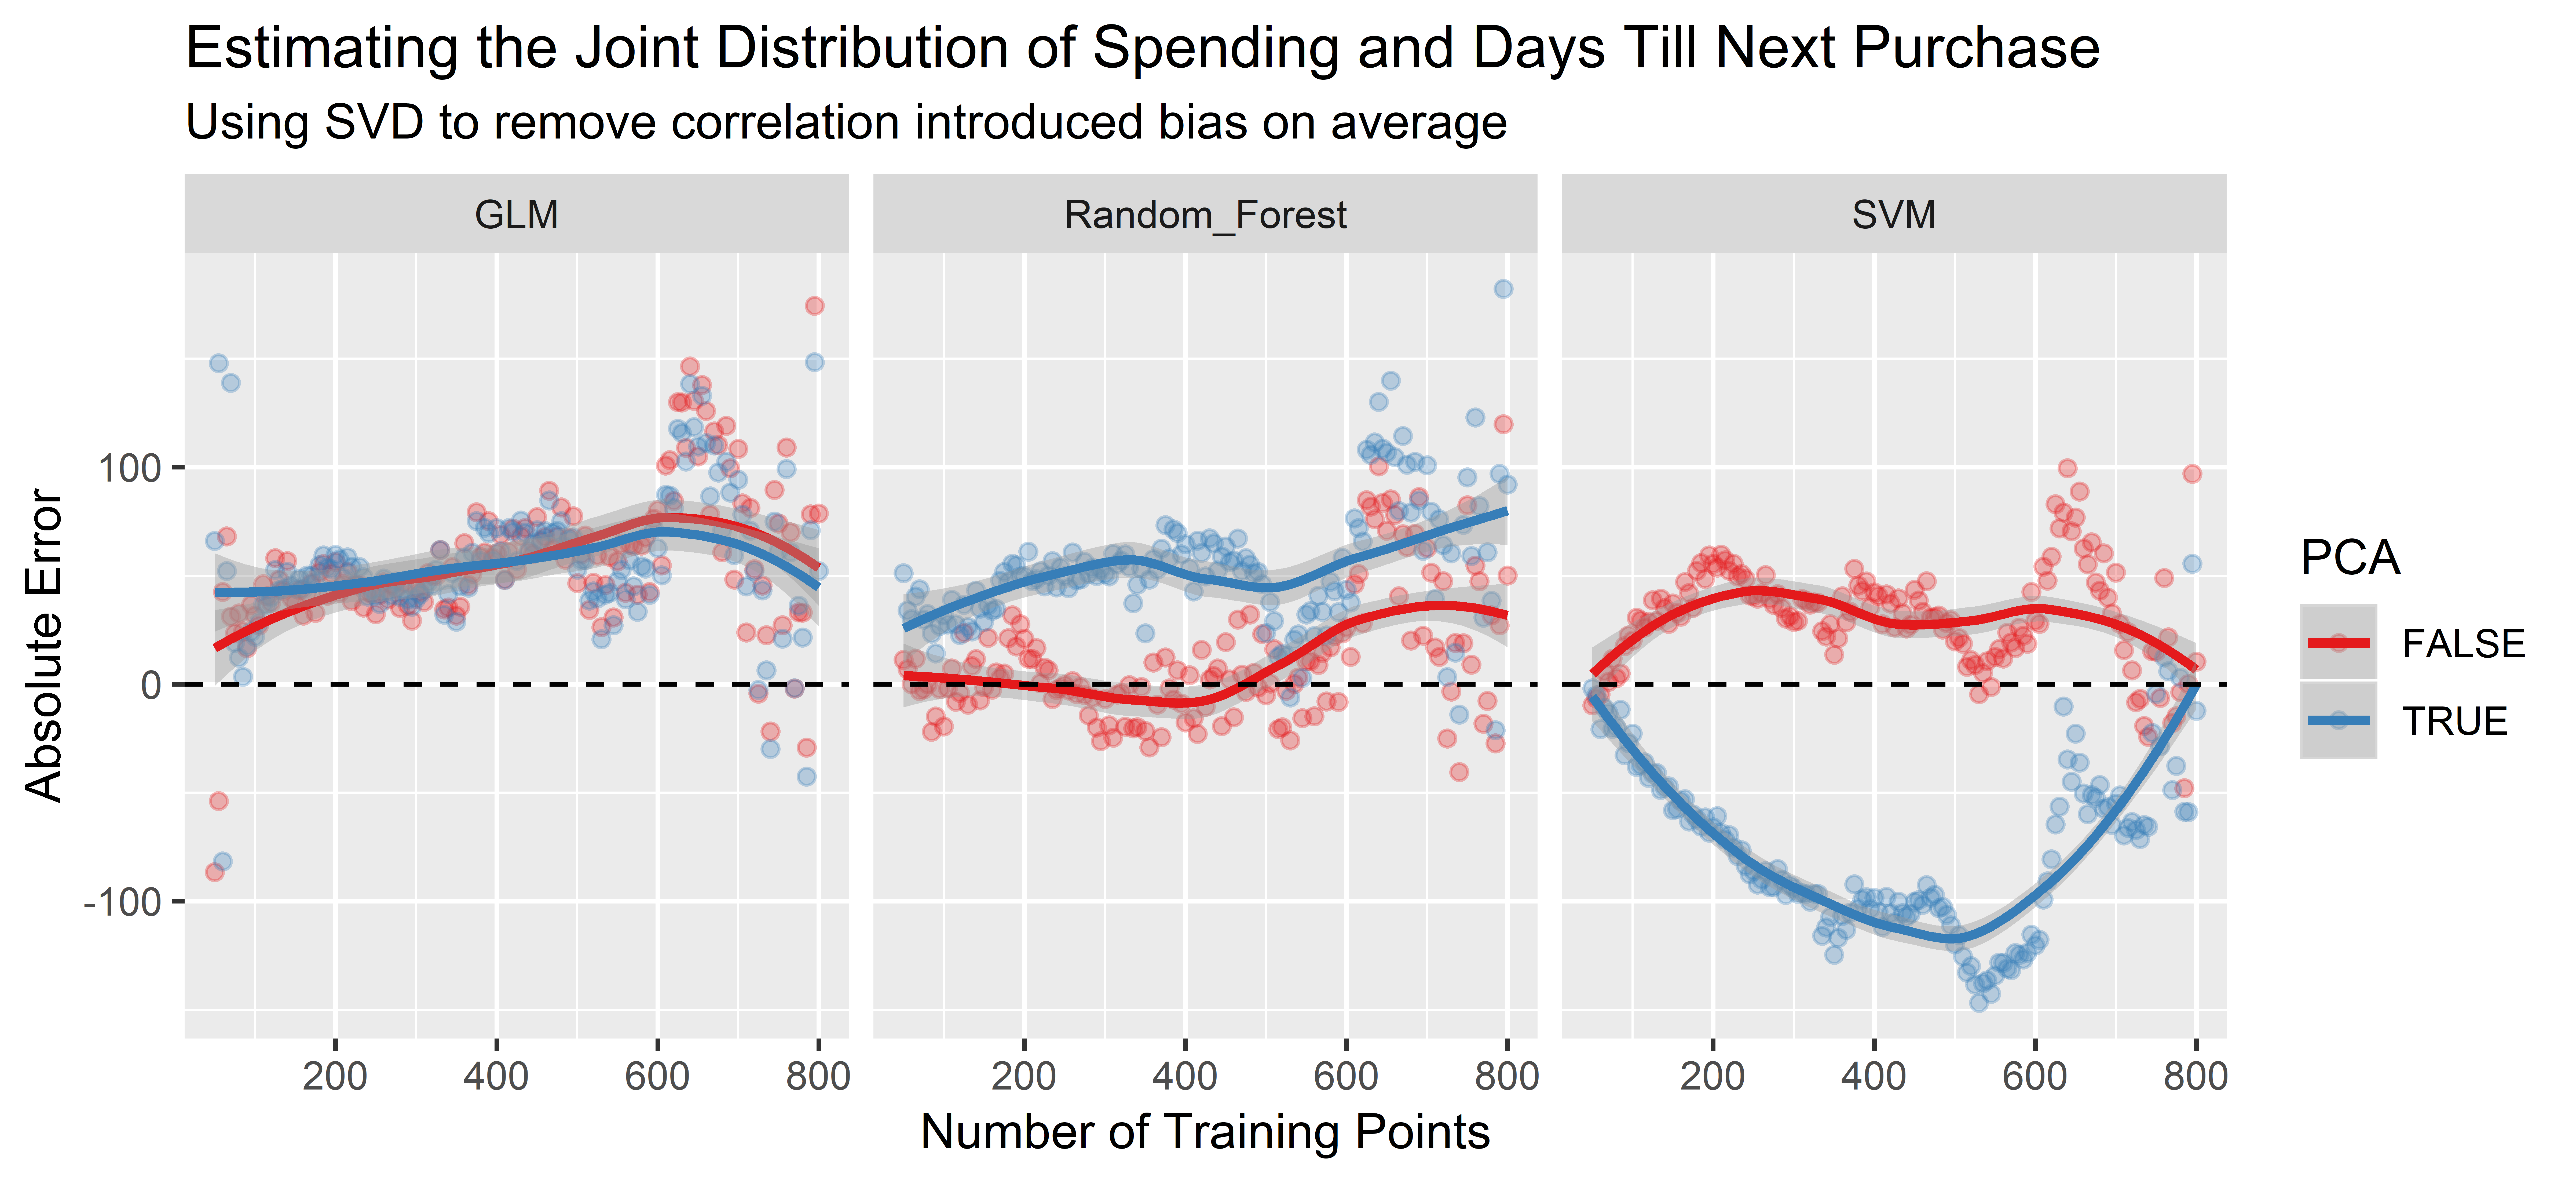
\includegraphics[width=1\linewidth]{../figures/07_yin_yang_multiple}
	\caption{Errors in prediction using the \yinyang style of prediction}
	\label{fig:07yinyangmultiple}
\end{figure}

The random forest is relatively unbiased, on the raw \yinyang data, from zero to almost 400 training points, while the PCA transformed data is systematically biased upwards.  The untransformed data predictions, being unbiased, is a surprising find. It shows that for up to almost a year of transactional data, the predictions are unbiased on average. While some of the averages exhibit autocorrelation, this was the first breakthrough in prediction with this data that I had and it was an indication that the prediction methods that I was using could be improved on.

The SVM algorithm is biased in both the raw and the transformed data. Like in the autocorrelation data, the SVM algorithm was not good in predicting the next value in the \yinyang series, and this was evident in the amount of bias that the algorithm exhibits when we look at the \bplots.  

\subsection{Most Promising Models}

After exploring a variety of combination of models, there were two models that outperformed compared to their peers. The first model was based on the Prophet Time Series Prediction algorithm from Facebook, and the second was the \yinyang prediction method using Random Forests. We can see the results of the best methods in Figure \ref{fig:mostpromisingmethods} . 


\begin{figure}
	\centering
	\includegraphics[width=1\linewidth]{../figures/most_promising_methods}
	\caption{\bplots of the two most promising methods. On the left is the \bplots of Facebook's prediction algorithm and the plot on the right is the \bplots of the \yinyang prediction algorithm }
	\label{fig:mostpromisingmethods}
\end{figure}


Facebook's Prophet algorithm is a Bayesian time series algorithm that accounts for daily or weekly seasonality, missing observations, outliers, and linear and non-linear trends. While I expected it to have a good performance in general, I expected the algorithm to struggle with the high amount of zeros in the dataset. However, as shown in the \bplots, we can see that it is a very effective algorithm, on average, for predicting the next months spending in an unbiased manner on average. 

The \yinyang prediction using Random Forests is also surprising in its performance. While it performs far better than Prophet on small training samples, it appears that it has more systemic bias than Prophet on average. 

In general, I would recommend using the \yinyang Random Forest strategy if the size of the training set is small and I would recommend using the Prophet strategy if the number of points to train on exceeds 100. With both algorithms, it is the case that they become biased with more training data. I think this is an artifact of the outliers in the data and these outliers can, in the short run, be averaged out using a small sample size. But, as the number of training points increases, we can see that the outliers bias the predictions upwards which results in the upward characteristic tails that we see in almost all of the \bplots in this paper. 




\section{Discussion}

For an end user, the largest consideration now, since we have discovered unbiased prediction methods, is to lessen the variance of the predictions. Since this paper focused predominately on the unbiased aspect of the \preprob, I think that the paper succeeded in its aim to produced unbiased estimators, the variance of the estimates is one of the aspects for an end user that I would like to control. 

The performance of the algorithms was surprising to me. I was not expecting to find algorithms that were unbiased over large domains of training data size, and I was not expecting an algorithm to work on the raw data like Prophet. Yet both of these things happened, and it was a cause for celebration that perhaps personal financial predictions are possible despite the various challenges with the data. 

The best methods strongly outperformed the baselines in the sense that they are largely unbiased and the variance of their estimates is less. However, the variance of the errors, for the average user, is still too large to be useful (the average error in prediction is still around 30\% which indicates that most estimates would still be difficult to hedge uncertainty with). 

I purposely did not choose to compute a metric on the performance outside of \bplots so that a user of the data would have to see the data as a whole and not as a set of summary statistics. The location and the trends in the bias, as as function of the number of training points, is critical to see in its totality without summarizing it down to numbers that do not portray these patterns. For this reason, I would recommend that a user of these prediction algorithms choose their algorithm of choice and use \bplots to decide between algorithm alternatives that suit their amount of training data and tolerances for error. 

\missingfigure{Take here going up}

\section{Things Left Undone}

Below is a list of the methods that are in consideration still for future development:
\begin{description}
	\item[Hidden Markov Models] I wanted to implement a fully Bayesian HMM that could be useful for sequence prediction in the personal financial time series. However, due to the difficulty in estimating the joint posterior of an HMM using the forward algorithm in determining the number of clusters, I abandoned this approach. Bayesian HMMs are a method I would like to visit in the future for estimation - especially for the \yinyang prediction system
	\item[Multivariate Regression] For the \yinyang Regression Problem, Multivariate Regression is something that I wanted to try as it allows us to predict both $ y_i $ and $ z_i $ jointly using the same algorithm. I only found out about these methods a week before the final submission of the project. In future research, I want to see if Multivariate Regression can outperform the marginal approach that did quite well with Random Forests. 
	\item[Neural Nets and LTSM] I wanted to use deep learning in some form, but I ran out of time in implementing them fully. Initial trails performance were so terrible in performance they were scrapped. The amount of data is so small and exhibits such extreme sparsity that the deep learning models may be too difficult to train. 
	\item[Loss Functions] I wanted to use different loss functions instead of just $ L_1 $ symmetric loss to judge the quality of the predictions of an algorithm. It is often more detrimental in these predictions to under-predict financial expenditures then to over-predict financial expenditures. An asymmetric loss function, that takes into account this asymmetric risk in prediction, would have been a great addition. Current candidates for loss functions are a multi-linear linear function such as 
	\begin{align*}
	L(x) = \begin{cases}
	\left|x\right| & \text{ for }  x \leq 0 \\
	m\left|x\right| & \text{ for }  x > 0, m > 1 
	\end{cases}
	\end{align*} which can be simplified as 
	\begin{align*}
	L(x) = \left(1 + m\mathbb{I}\left[x > 0\right]\right)\left|x\right|
	\end{align*} or 
	\begin{align*}
	L(x) = \max\left\lbrace 0, x \right\rbrace
	\end{align*} Asymmetric Pseudo Huber Loss\footnote{A good introduction to Huber Loss can be found here: \url{https://en.wikipedia.org/wiki/Huber_loss}} would also be a great alternative which is given by
	\begin{align*}
	\zeta &=  \left(1 + m\mathbb{I}\left[x > 0\right]\right) \\
	L_\delta(x) &= \zeta \delta^2 \left(\sqrt{1 + \left(\frac{x}{\delta}\right)^2} - 1\right)
	\end{align*}
	where the loss is both convex (an advantage of $ L_2 $ loss) while not being as extreme for a loss far from zero. $ \delta $ is a parameter that tells the loss where the shift from highly convex to linear loss should occur.
	\item[Stacked Models] To reduce the variance of the estimates, I want to build up a stacked model. A stacked model takes the output of several algorithms trained on the data and uses their predictions as covariates for its own prediction. I envision that the correlation of the errors could create problems for a stacked approach, but I would like to consider it nevertheless in the future.  
	\item[Visualization Metrics] From the inception of the project, the goal was to create a series of visualizations that could be used to convey, to the average user, the current status of their financial future. Bullet Charts, from Stephen Few, are something that I wanted to experiment with to discern if the average user would find them useful for a dashboard view of their finances. I have implemented some visualizations for my personal data, but I was not able to polish them enough to make the final report. Among the visualizations I wanted to create, I wanted to implement a Monthly Spending index as well. This visualization I would like to devote some time to in the future. 
	\item[More "Cooks in the Kitchen"] Discovery is hard. While sometimes multiple coders can run into each other, it would have been amazing to have a few more "cooks in the kitchen" to bounce ideas off of and test other prediction methods. While novel methods were presented and unbiased predictors were discovered, another coder to implement the dozen or so coding files, develop graphics, process data, and improve on predictions would have been a great help. 
\end{description}

\section{Work Plan}

I set out to create an unbiased predictor of monthly spending for personal financial data and to create visualization and metrics that a user could use that would be able to inform them on their financial health. With regards to the prediction task, I think that I achieved the first step of what I set out to do. Given the difficulty of the data, this was not a small task. 

However, in terms of importance, I believe that the visualization aspect of the project was as important, or even more important, than the prediction component. Users interact with visualizations, and in terms of business purpose, the visualizations are something that I would like to continue to flesh out. This is only the start of what is likely to be a multi-year project, and I am excited to explore more on the visualization side as the project progresses. 

\section*{Acknowledgments}

I would like to thank my brother, Cameron Kurzeja, my time working in banking, and the creators of YNAB\footnote{YNAB is an excellent budgeting software that made the data collection for this project possible}, for creating the perfect storm that inspired this project and made it possible. 


% include your own bib file like this:
\bibliography{references}
\bibliographystyle{acl_natbib}


\end{document}
